% Szglab4
% ===========================================================================
%
\chapter{Grafikus felület specifikációja}

\thispagestyle{fancy}

\section{A grafikus interfész}
\comment{A menürendszer, a kezelői felület grafikus képe. A grafikus felület megjelenését, a használt ikonokat, stb screenshot-szerű képekkel kell bemutatni. Az építészetben ez a homlokzati terv.}

A játék indításakor az alábbi menü jön be:

\begin{figure}[H]
	\begin{center}
		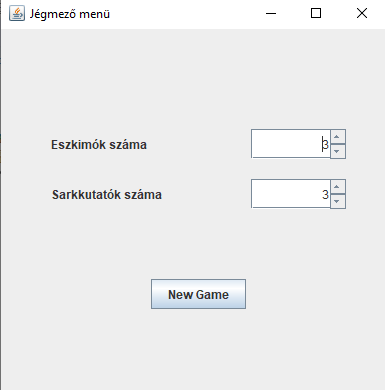
\includegraphics[width=11cm]{chapters/chapter11/res/menu.png}
		\caption{A játék menüjét bemutató ábra}
		\label{fig:Menu}
	\end{center}
\end{figure}

A két Spinner segítségével kiválasztható a játékosok száma, kutatókra és eszkimókra lebontva.
A New Game gomb segítségével indítható el a játék, ami működés közben valahogy így néz ki:

\begin{figure}[H]
	\begin{center}
		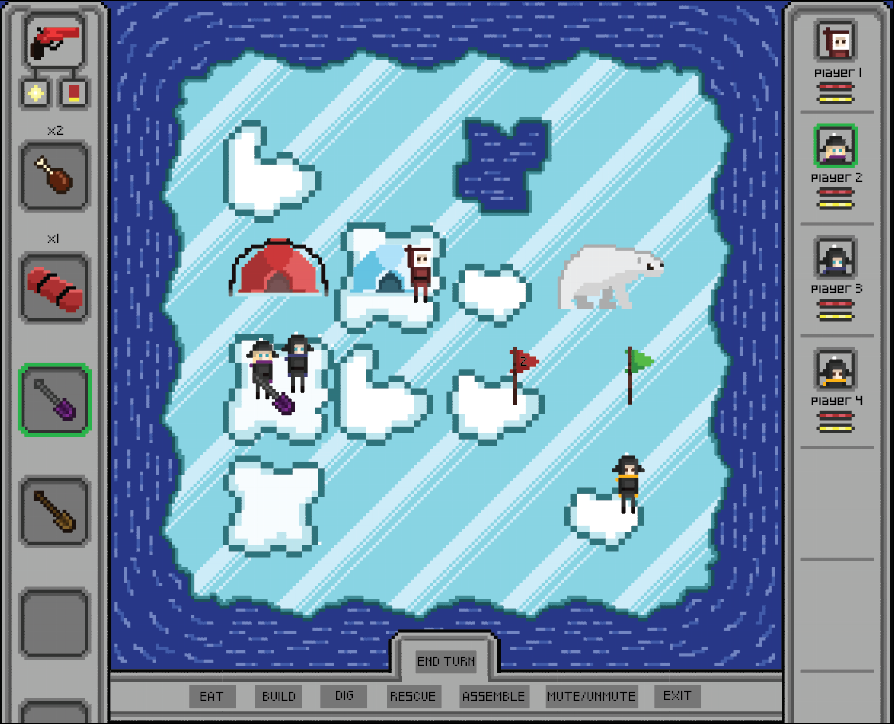
\includegraphics[width=11cm]{chapters/chapter11/res/game1.png}
		\caption{Kép a játékról, eszközökkel}
		\label{fig:Game1}
	\end{center}
\end{figure}
\begin{figure}[H]
	\begin{center}
		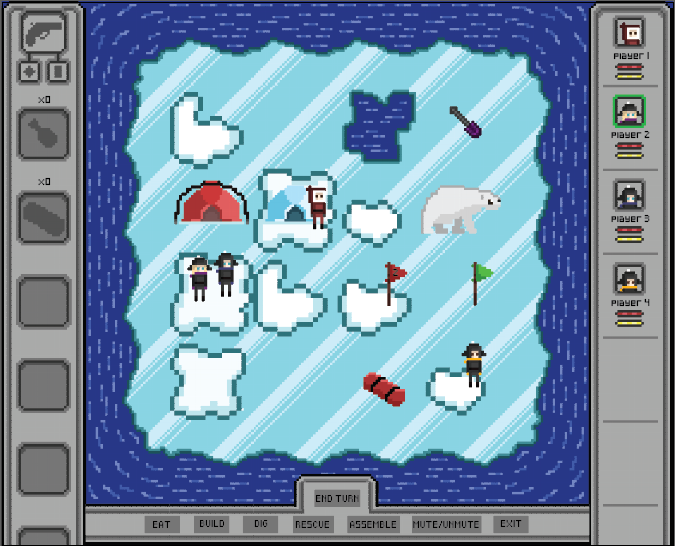
\includegraphics[width=11cm]{chapters/chapter11/res/game2.png}
		\caption{Kép a játékról, eszközök nélkül}
		\label{fig:Game2}
	\end{center}
\end{figure}

A képen láthatók a játékosok jobb oldalt, akik részt vesznek a játékban. Az ikonjuk alapján megkülönböztethetőek egyértelműen. Az ikon alatt pirossal a testhő, sárgával a játékos energiája látható.
Az aktuálisan kiválasztott játékost, akit zöld keret vesz körül, lehet irányítani, és láthatóak a tárgyai a bal oldalon. Az éppen használatban lévő tárgyakat szintén zöld keret veszi körül. Az élelem és sátorzacskó fogyócikkek fölött számláló helyezkedik el, ami a kiválasztott játékosnak éppen birtokában lévő mennyiséget jelzi belőlük. A tárgyak között látható törékeny falapát, míg törhetetlen lila kristálylapát is.
A képernyő alján az akciógombok helyezkednek el, ezekkel lehet a modellben specifikált use-casek szerint irányítani az éppen kiválasztott játékost. Emellett ha már nem szeretne akciót végezni, véget vethet körének a játékos. A játékból való kilépés és a hang kikapcsolása is ezen a gombsoron kapott helyet.
A képernyő közepén található a lényeg, maga a játék megjelenítése. A jégmezőt a hideg, fagyos óceán veszi körül, míg a tükörsima jégen félelmetes jegesmedve szörny, és tőle rettegő, onnan menekülni vágyó játékosok láthatók. Kapucniban az iglulakó eszkimók találhatók, míg sapkában a sarkkutatók fedezik fel a jégtáblák rejtelmeit. Felfedezett jégtábláik teherbírását zászlóval jelölik: zölddel, ha az nem törhet el, míg pirossal és egy számmal, ha az eltörhet a számot meghaladó játékosok lába alatt.
A jégen találhatók tárgyak is, sátorzacskó, törhetetlen lapát, emellett vannak épületek is lerakva, iglu és sátor is.
A jégmezőn található hóval nem fedett vizesgödör, hóval fedett és sima jégtábla is. A hómennyiség az üres jégtől kezdve 5 réteg hóig terjedhet, mindegyik látható a pillanatképünkön.
A jégmezőn néha feltámad a hóvihar, ez az alábbihoz hasonló animációval lesz majd megjelenítve:

\begin{figure}[H]
	\begin{center}
		
\includegraphics[width=11cm]{chapters/chapter11/res/storm.png}
		\caption{Kép a játékban a hóviharról}
		\label{fig:Snowstorm}
	\end{center}
\end{figure}

\section{A grafikus rendszer architektúrája}
\comment{A felület működésének elve, a grafikus rendszer architektúrája (struktúra diagramok). A struktúra diagramokon a prototípus azon és csak azon osztályainak is szerepelnie kell, amelyekhez a grafikus felületet létrehozó osztályok kapcsolódnak.}

\subsection{A felület működési elve}

A feladat megvalósítása során törekedtünk az MVC architechtúrára. A modellt a korábbi fázisokban elkészült program biztosítja. A modell önmagában csak adatokat szogláltat ezért minden adata hozzáférhető getterek segítségével. A View pullolja a modell adatait, míg a Controller pusholja azt. A modell önmagában nem observable, mert minden változást a Controller vált ki futása során.

A View egy pálya nézet. Megkapja a Modellt mint dependecy injection. Update hatására kiolvassa a Modell álapotát és megjeleníti azt. A View implementálja a GameObservert.

A Controller felelős a UI elemek kezeléséért. Megkapja a Modell-t és a View-t, mint dependency injection. Feliratkozhat a View eventjeire, ha az is irányítható. Fontos feladata az felhasználótól érkező inputok lekezelése. Írja a modell álapotát, frissíti a View-t.

A főprogram felelős a játék főmenüjének megjelenítéséért és az ehhez kapcsolódó inputok lekezeléséért. A főmenüben meg lehet adni a játékosok számát, neveit. Modellt épít a Proto-val. Implementálja a GameObserver-t, ezzel képes a játék végét kezelni. View-t és Controller-t nyit és zár.
\subsection{A felület osztály-struktúrája}

\begin{figure}[H]
	\begin{center}
		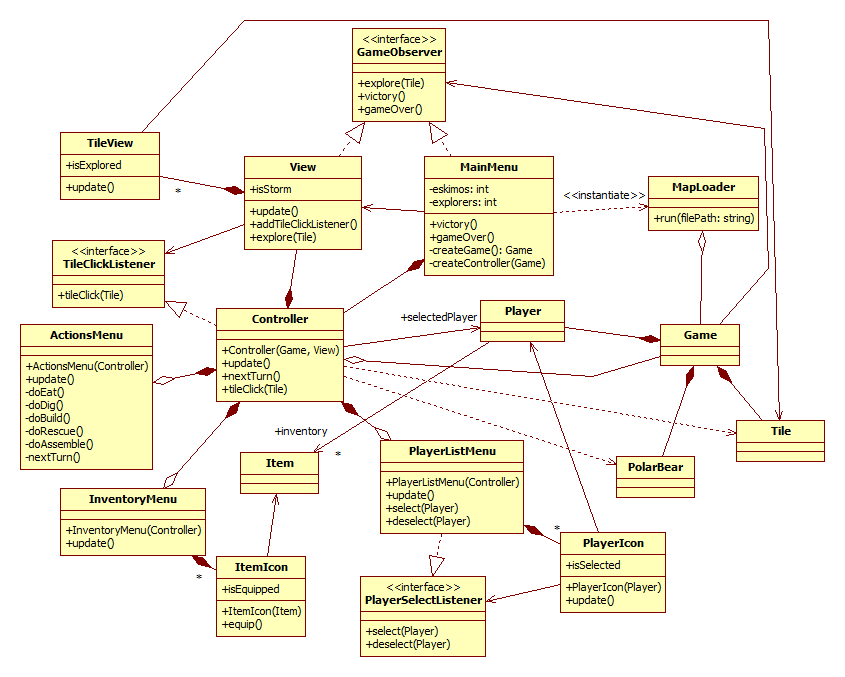
\includegraphics[width=17cm]{chapters/chapter11/classdiagram.png}
		\caption{Classdiagram az új osztályokról}
		\label{fig:classdiagram}
	\end{center}
\end{figure}

\section{A grafikus objektumok felsorolása}

\subsection{View}
\begin{itemize}
\item Felelősség\newline
Felelőssége a játékpálya megjelenítése és felépítése. A játékpálya TileView-k ból épül majd fel.
\item Ősosztályok\newline
JScrollPane
\item Interfészek\newline
MouseListener GameObserver
\item Attribútumok\newline
	\begin{itemize}
		\item isStorm: bool: Havazik-e a pályán +
	\end{itemize}
\item Metódusok\newline
	\begin{itemize}
		\item void update(): Frissíti a tábla elemeit. +
		\item void addTileClickedListener(TileClickedListener tcl): Szól neki ha a TileView-ra klikkeltek +
		\item void explore(Tile t): Beállítja a megdfelelő TileView.isExplored-et. +
	\end{itemize}
\end{itemize}

\subsection{TileClickedListener}
\begin{itemize}
	\item Felelősség\newline
	Figyeli a kattintást a tilen. Interfész
\end{itemize}

\subsection{TileView}
\begin{itemize}
	\item Felelősség\newline
	Felelős egy tile kirajzolásáért.
	\item Ősosztályok\newline
	JPanel
	\item Attribútumok\newline
	\begin{itemize}
		\item tile: Tile: Maga a tile amit ismer -
		\item isExplored: bool: Felderítették-e. +
	\end{itemize}
	\item Metódusok\newline
	\begin{itemize}
		\item void update(): Kiolvassa a Tile információit és rajzol. +
	\end{itemize}
\end{itemize}

\subsection{Controller}
\begin{itemize}
	\item Felelősség\newline
	Felelőssége az Modell és a View közötti kapcsolat megteremtése. Kezeli a modell adatait érzékeli a view-n megadott inputokat.
	\item Ősosztályok\newline
	JFrame
	\item Interfészek\newline
	TileClickListener
	\item Attribútumok\newline
	\begin{itemize}
		\item selectedPlayer: Player: Első játákos/kiválasztott +
		\item game: Game: Maga a játék instance, modell. +
		\item view: View: A tartalmazott View osztály amit megjelenít. +
		\item inventoryMenu: InventoryMenu: Ez az oldalt megjelenített sáv. +
		\item actionsMenu: ActionsMenu: Az alul megjelenített gomb sáv. +
		\item playerList: PlayerList: Játékosok listája. +	
	\end{itemize}
	\item Metódusok\newline
	\begin{itemize}
		\item void update(): Frissíti az összes grafikai elemet. +
		\item void nextTurn(): Egy kör lefutását kezeli. +
		\item void tileClick(Tile t): Ha a cella szomszédos a jelenleg kiválasztott játékossal akkor odalép. +
	\end{itemize}
\end{itemize}

\subsection{InventoryMenu }
\begin{itemize}
	\item Felelősség\newline
	Felelőssége kezelni az oldalt megjelenített tároló panelt.
	\item Ősosztályok\newline
	JPanel
	\item Attribútumok\newline
	\begin{itemize}
		\item controller: Controller: Ismeri a hozzá tartozó vezérlőt. +	
	\end{itemize}
	\item Metódusok\newline
	\begin{itemize}
		\item void update(): Frissíti az itemiconokat. +
	\end{itemize}
\end{itemize}

\subsection{ItemIcon}
\begin{itemize}
	\item Felelősség\newline
	Mutat egy itemet, számosságot, mutatja, hogy equippelve van.
	\item Ősosztályok\newline
	JPanel
	\item Interfészek\newline
	MouseListener
	\item Attribútumok\newline
	\begin{itemize}
		\item item: Item: Milyen tárgyról van szó +
		\item controller: Controller: Ismeri a hozzá tartozó vezérlőt. +	
		\item isEquipped: bool: Kézben van-e éppen. +
	\end{itemize}
	\item Metódusok\newline
	\begin{itemize}
		\item void equip(): Equipped állapot beállítása. +
	\end{itemize}
\end{itemize}

\subsection{ActionsMenu}
\begin{itemize}
	\item Felelősség\newline
	Kezeli a műveleti gombok működését.
	\item Ősosztályok\newline
	JPanel
	\item Interfészek\newline
	ActionListener
	\item Attribútumok\newline
	\begin{itemize}
		\item controller: Controller: Ismeri a hozzá tartozó vezérlőt. +	
	\end{itemize}
	\item Metódusok\newline
	\begin{itemize}
		\item void update(): Frissíti a gombokat megnyomásukkor, figyeli melyik lehet aktív az adott eszközök alapján. +
		\item void doDig(): Ásás gomb esemény. +
		\item void doBuild(): Iglu/sátor gomb esemény. +
		\item void doEat(): Evés gomb esemény. +
		\item void doRescue(): Kimentés gomb esemény. +
		\item void doAssemble(): Pisztoly építés gomb esemény. +
		\item void exit(): Kilépés. +
		\item void nextTurn(): Következő kör gomb esemény. +
	\end{itemize}
\end{itemize}

\subsection{PlayerList}
\begin{itemize}
	\item Felelősség\newline
	PlayerIconok függőleges listája
	\item Ősosztályok\newline
	JPanel
	\item Interfészek\newline
	PlayerSelectListener
	\item Attribútumok\newline
	\begin{itemize}
		\item controller: Controller: Ismeri a hozzá tartozó vezérlőt. +	
	\end{itemize}
	\item Metódusok\newline
	\begin{itemize}
		\item void update(): Kiválasztott játékos panel frissítése. +
	\end{itemize}
\end{itemize}

\subsection{PlayerIcon}
\begin{itemize}
	\item Felelősség\newline
	Mutatja a Player ikonját, nevét, testhőjét, energiáját
	\item Ősosztályok\newline
	JPanel
	\item Interfészek\newline
	MouseListener
	\item Attribútumok\newline
	\begin{itemize}
		\item controller: Controller: Ismeri a hozzá tartozó vezérlőt. +	
		\item player: Player: Maga a játékos. +
		\item isSelected: bool: kivan kiválasztva. +
	\end{itemize}
	\item Metódusok\newline
	\begin{itemize}
		\item void update(): Kiválasztott játékos panel frissítése. +
	\end{itemize}
\end{itemize}

\subsection{PlayerSelectListener }
\begin{itemize}
	\item Felelősség\newline
	Interfész, kezeli a kiválasztást.
\end{itemize}

\subsection{Main}
\begin{itemize}
	\item Felelősség\newline
	Belépési pont.
	\item Metódusok\newline
	\begin{itemize}
		\item void main(): Fő szál. +
	\end{itemize}
\end{itemize}

\subsection{MainMenu}
\begin{itemize}
	\item Felelősség\newline
	Főmenü működése.
	\item Ősosztályok\newline
	JFrame
	\item Interfészek\newline
	WindowAdapter, ActionListener, GameObserver
	\item Attribútumok\newline
	\begin{itemize}
		\item controller: Controller: Ismeri a hozzá tartozó vezérlőt. +	
		\item numEskimos: int: Eszkimók száma. +
		\item numExplorers: int: PolarExplorererk száma. +	
	\end{itemize}
	\item Metódusok\newline
	\begin{itemize}
		\item void victory(): Játék vége. +
		\item void gameOver(): Játék vége. +
		\item Game createGame(): Játék létrehozása. -
		\item Controller createController(Game g): Controller létrehozása. -
	\end{itemize}
\end{itemize}

\subsection{MapLoader}
\begin{itemize}
\item Felelősség\newline
Pálya betöltése
\item Metódusok\newline
	\begin{itemize}
		\item void run(filePath: string): Utasítások betöltése fájlból. +
	\end{itemize}
\end{itemize}

\section{Kapcsolat az alkalmazói rendszerrel}
\comment{Szekvencia-diagramokon ábrázolni kell a grafikus rendszer működését. Konzisztens kell legyen az előző alfejezetekkel. Minden metódus, ami ott szerepel, fel kell tűnjön valamelyik szekvenciában. Minden metódusnak, ami szekvenciában szerepel, szereplnie kell a valamelyik osztálydiagramon.}

\begin{figure}[H]
	\begin{center}
		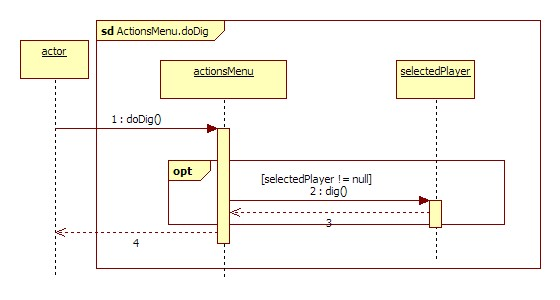
\includegraphics[width=10cm]{chapters/chapter11/seq/ActionMenu_doDig.jpg}
		\caption{ActionMenu Dig}
		\label{ActionMenu Dig}
	\end{center}
\end{figure}
\begin{figure}[H]
	\begin{center}
		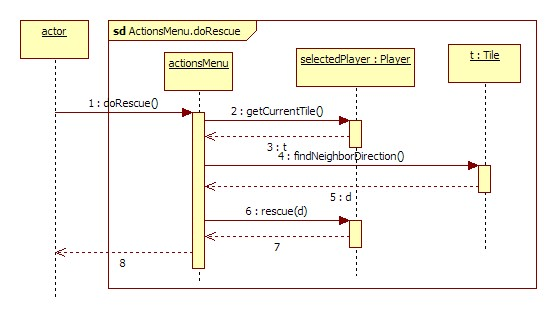
\includegraphics[width=10cm]{chapters/chapter11/seq/ActionMenu_doRescue.jpg}
		\caption{ActionMenu Rescue}
		\label{ActionMenu Rescue}
	\end{center}
\end{figure}
\begin{figure}[H]
	\begin{center}
		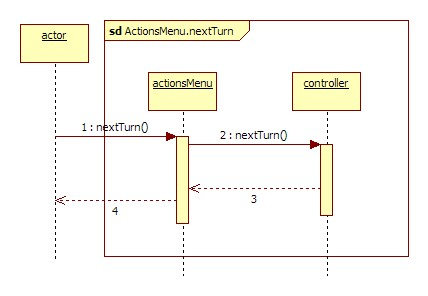
\includegraphics[width=10cm]{chapters/chapter11/seq/ActionsMenu.nextTurn.jpg}
		\caption{ActionMenu nextTurn}
		\label{ActionMenu nextTurn}
	\end{center}
\end{figure}
\begin{figure}[H]
	\begin{center}
		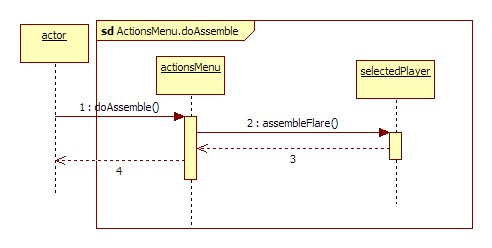
\includegraphics[width=10cm]{chapters/chapter11/seq/ActionsMenu_doAssemble.jpg}
		\caption{ActionMenu Assemble}
		\label{ActionMenu Assemble}
	\end{center}
\end{figure}
\begin{figure}[H]
	\begin{center}
		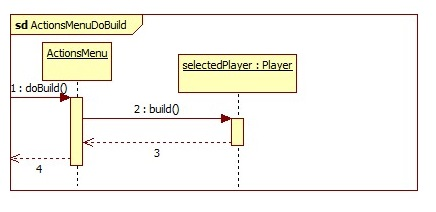
\includegraphics[width=10cm]{chapters/chapter11/seq/ActionsMenu_DoBuild.jpg}
		\caption{ActionMenu Build}
		\label{ActionMenu Build}
	\end{center}
\end{figure}
\begin{figure}[H]
	\begin{center}
		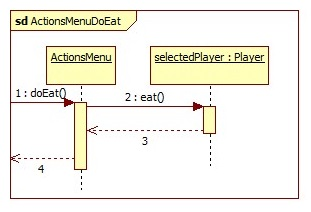
\includegraphics[width=10cm]{chapters/chapter11/seq/ActionsMenu_DoEat.jpg}
		\caption{ActionMenu Eat}
		\label{ActionMenu Eat}
	\end{center}
\end{figure}
\begin{figure}[H]
	\begin{center}
		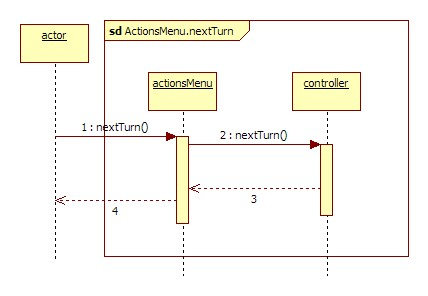
\includegraphics[width=10cm]{chapters/chapter11/seq/ActionsMenu.nextTurn.jpg}
		\caption{ActionMenu nextTuirn}
		\label{ActionMenu nextTurn}
	\end{center}
\end{figure}
\begin{figure}[H]
	\begin{center}
		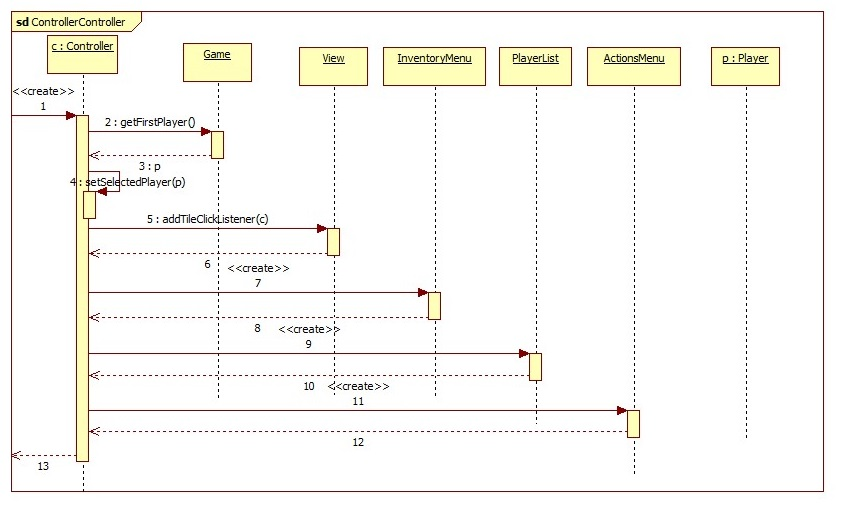
\includegraphics[width=10cm]{chapters/chapter11/seq/Controller_Controller.jpg}
		\caption{Controller init}
		\label{Controller init}
	\end{center}
\end{figure}
\begin{figure}[H]
	\begin{center}
		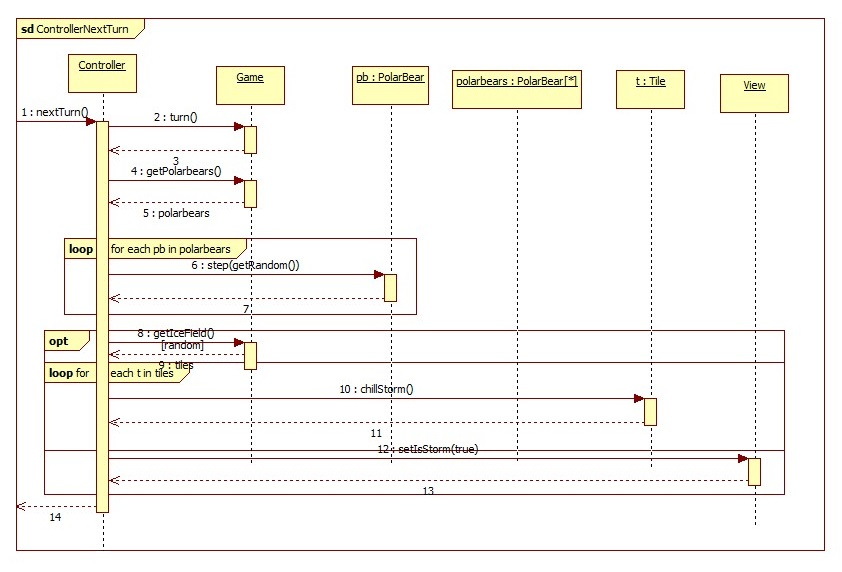
\includegraphics[width=10cm]{chapters/chapter11/seq/Controller_NextTurn.jpg}
		\caption{Controller nextTuirn}
		\label{Controller nextTurn}
	\end{center}
\end{figure}
\begin{figure}[H]
	\begin{center}
		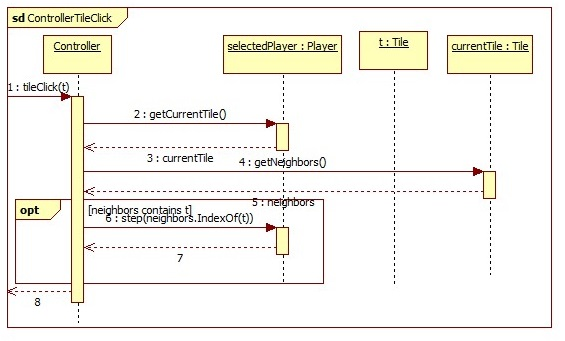
\includegraphics[width=10cm]{chapters/chapter11/seq/Controller_TileClick.jpg}
		\caption{Controller TileClick}
		\label{Controller TileClick}
	\end{center}
\end{figure}
\begin{figure}[H]
	\begin{center}
		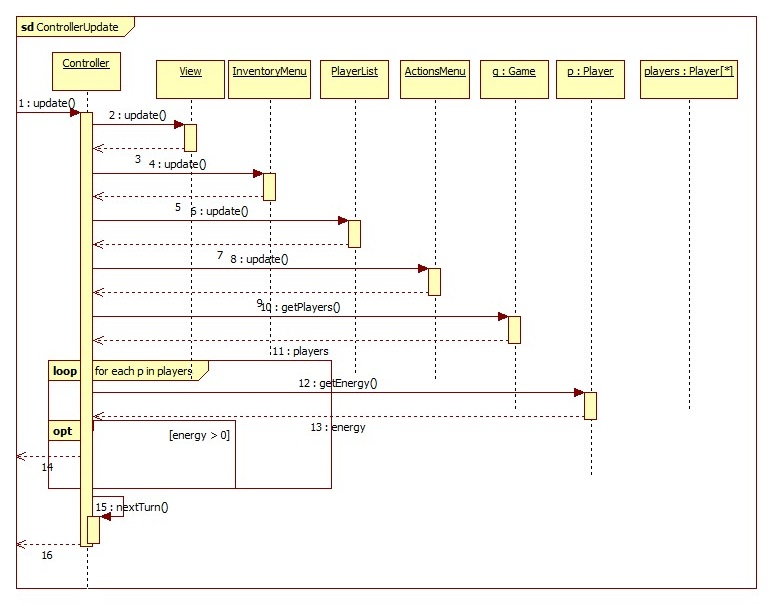
\includegraphics[width=10cm]{chapters/chapter11/seq/Controller_Update.jpg}
		\caption{Controller Update}
		\label{Controller Update}
	\end{center}
\end{figure}
\begin{figure}[H]
	\begin{center}
		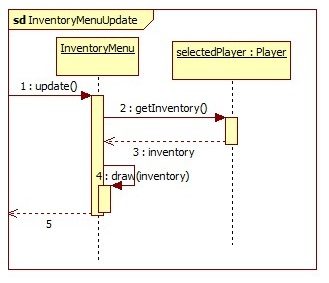
\includegraphics[width=10cm]{chapters/chapter11/seq/InventoryMenu_Update.jpg}
		\caption{InventoryMenu Update}
		\label{InventoryMenu Update}
	\end{center}
\end{figure}
\begin{figure}[H]
	\begin{center}
		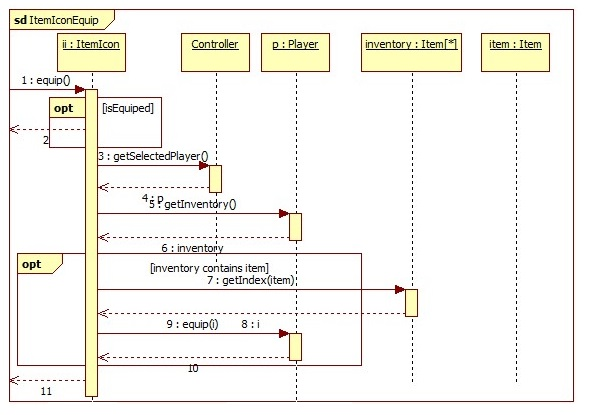
\includegraphics[width=10cm]{chapters/chapter11/seq/ItemIcon_Equip.jpg}
		\caption{ItemIcon Equip}
		\label{ItemIcon Equip}
	\end{center}
\end{figure}
\begin{figure}[H]
	\begin{center}
		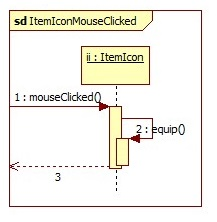
\includegraphics[width=10cm]{chapters/chapter11/seq/ItemIcon_MouseClicked.jpg}
		\caption{ItemIcon MouseClicked}
		\label{ItemIcon MouseClicked}
	\end{center}
\end{figure}
\begin{figure}[H]
	\begin{center}
		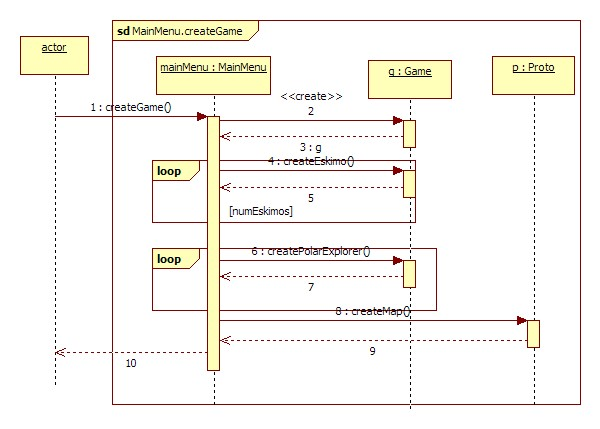
\includegraphics[width=10cm]{chapters/chapter11/seq/MainMenu_createGame.jpg}
		\caption{MainMenu CreateGame}
		\label{MainMenu CreateGame}
	\end{center}
\end{figure}
\begin{figure}[H]
	\begin{center}
		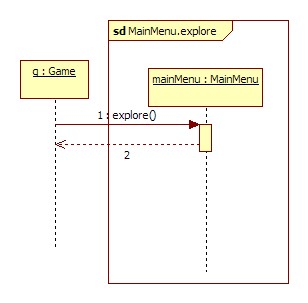
\includegraphics[width=10cm]{chapters/chapter11/seq/MainMenu_explore.jpg}
		\caption{MainMenu Explore}
		\label{MainMenu Explore}
	\end{center}
\end{figure}
\begin{figure}[H]
	\begin{center}
		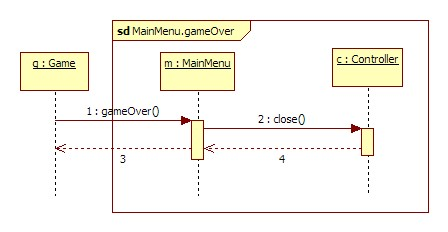
\includegraphics[width=10cm]{chapters/chapter11/seq/MainMenu_gameOver.jpg}
		\caption{MainMenu GameOver}
		\label{MainMenu GameOver}
	\end{center}
\end{figure}
\begin{figure}[H]
	\begin{center}
		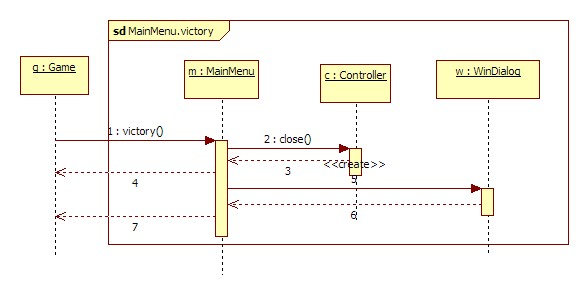
\includegraphics[width=10cm]{chapters/chapter11/seq/MainMenu_victory.jpg}
		\caption{MainMenu Victory}
		\label{MainMenu Victory}
	\end{center}
\end{figure}
\begin{figure}[H]
	\begin{center}
		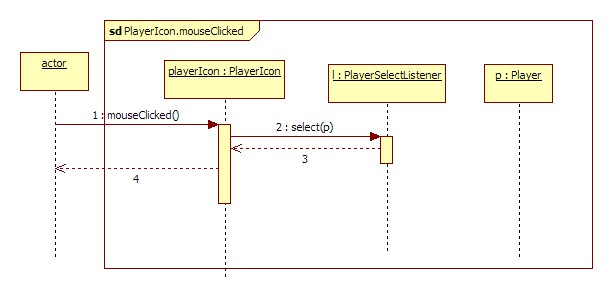
\includegraphics[width=10cm]{chapters/chapter11/seq/PlayerIcon_mouseClicked.jpg}
		\caption{PlayerIcon MouseClicked}
		\label{PlayerIcon MouseClicked}
	\end{center}
\end{figure}
\begin{figure}[H]
	\begin{center}
		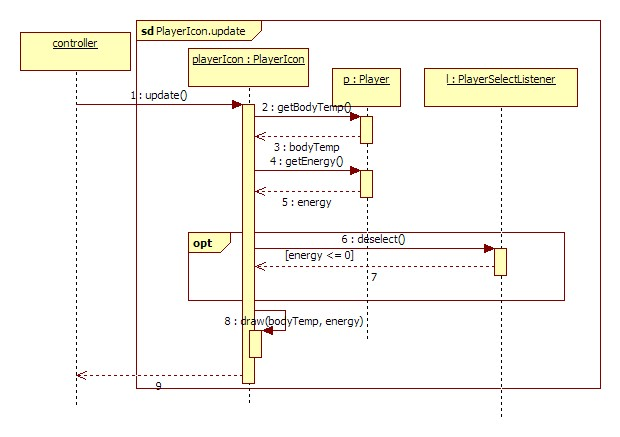
\includegraphics[width=10cm]{chapters/chapter11/seq/PlayerIcon_update.jpg}
		\caption{PlayerIcon Update}
		\label{PlayerIcon Update}
	\end{center}
\end{figure}
\begin{figure}[H]
	\begin{center}
		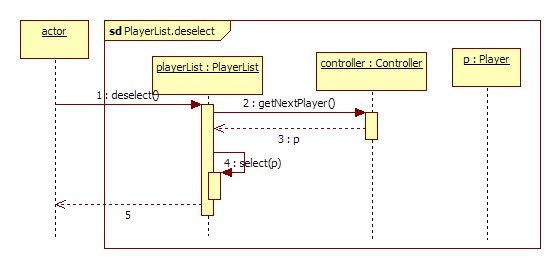
\includegraphics[width=10cm]{chapters/chapter11/seq/PlayerList_deselect.jpg}
		\caption{PlayerList Deselect}
		\label{PlayerList Deselect}
	\end{center}
\end{figure}
\begin{figure}[H]
	\begin{center}
		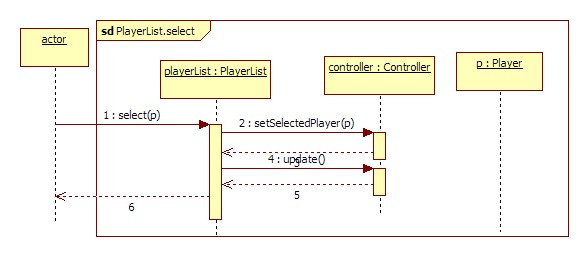
\includegraphics[width=10cm]{chapters/chapter11/seq/PlayerList_select.jpg}
		\caption{PlayerList Select}
		\label{PlayerList Select}
	\end{center}
\end{figure}
\begin{figure}[H]
	\begin{center}
		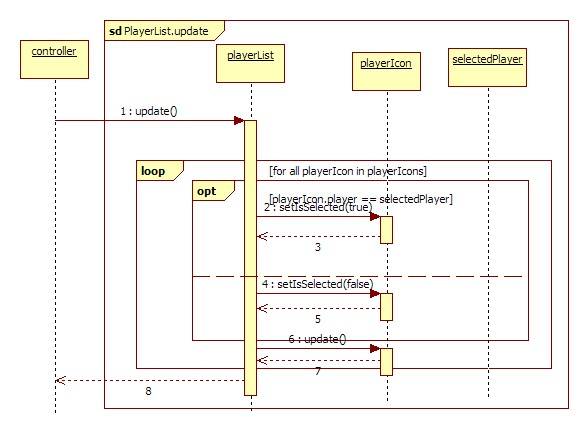
\includegraphics[width=10cm]{chapters/chapter11/seq/PlayerList_update.jpg}
		\caption{PlayerList Update}
		\label{PlayerList Update}
	\end{center}
\end{figure}
\begin{figure}[H]
	\begin{center}
		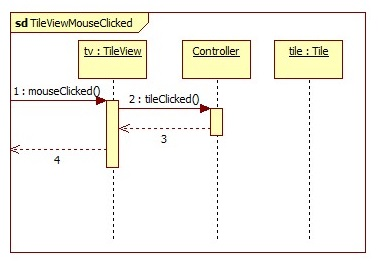
\includegraphics[width=10cm]{chapters/chapter11/seq/TileView_MouseClicked.jpg}
		\caption{TileView MouseClicked}
		\label{TileView MouseClicked}
	\end{center}
\end{figure}
\begin{figure}[H]
	\begin{center}
		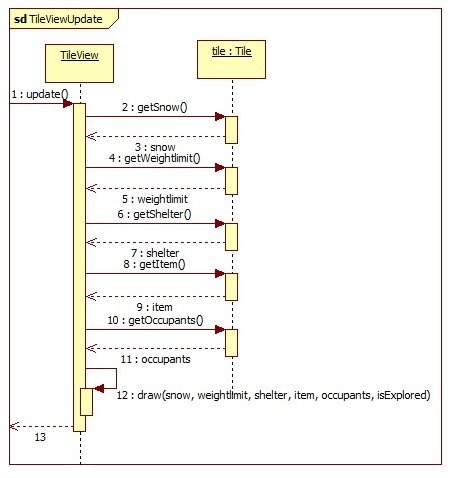
\includegraphics[width=10cm]{chapters/chapter11/seq/TileView_Update.jpg}
		\caption{TileView Update}
		\label{TileView Update}
	\end{center}
\end{figure}
\begin{figure}[H]
	\begin{center}
		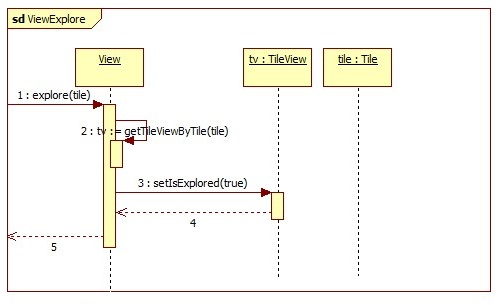
\includegraphics[width=10cm]{chapters/chapter11/seq/View_Explore.jpg}
		\caption{View Explore}
		\label{View Explore}
	\end{center}
\end{figure}
\begin{figure}[H]
	\begin{center}
		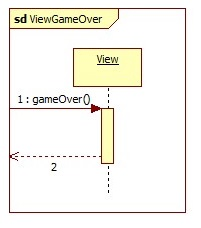
\includegraphics[width=10cm]{chapters/chapter11/seq/View_GameOver.jpg}
		\caption{View GameOver}
		\label{View GameOver}
	\end{center}
\end{figure}
\begin{figure}[H]
	\begin{center}
		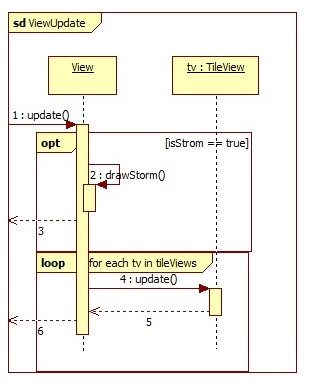
\includegraphics[width=10cm]{chapters/chapter11/seq/View_Update.jpg}
		\caption{View Update}
		\label{View Update}
	\end{center}
\end{figure}
\begin{figure}[H]
	\begin{center}
		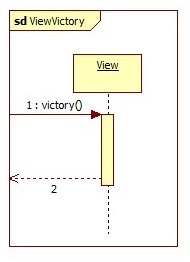
\includegraphics[width=10cm]{chapters/chapter11/seq/View_Victory.jpg}
		\caption{View Victory}
		\label{View Victory}
	\end{center}
\end{figure}


